\documentclass{aa}

\usepackage{graphicx}

\usepackage[varg]{txfonts}
\usepackage{units}
\usepackage{mathtools}
\usepackage{color}
\usepackage{natbib,twoopt}
\usepackage{siunitx}
\usepackage{hyperref} %% to avoid \citeads line fills
\bibpunct{(}{)}{;}{a}{}{,}             %% natbib format for A&A and ApJ
\makeatletter
  \newcommandtwoopt{\citeads}[3][][]{\href{http://adsabs.harvard.edu/abs/#3}%
    {\def\hyper@linkstart##1##2{}%
     \let\hyper@linkend\@empty\citealp[#1][#2]{#3}}}
  \newcommandtwoopt{\citepads}[3][][]{\href{http://adsabs.harvard.edu/abs/#3}%
    {\def\hyper@linkstart##1##2{}%
     \let\hyper@linkend\@empty\citep[#1][#2]{#3}}}
  \newcommandtwoopt{\citetads}[3][][]{\href{http://adsabs.harvard.edu/abs/#3}%
    {\def\hyper@linkstart##1##2{}%
     \let\hyper@linkend\@empty\citet[#1][#2]{#3}}}
  \newcommandtwoopt{\citeyearads}[3][][]%
    {\href{http://adsabs.harvard.edu/abs/#3}
    {\def\hyper@linkstart##1##2{}%
     \let\hyper@linkend\@empty\citeyear[#1][#2]{#3}}}
  \renewcommand*\aa@pageof{, page \thepage{} of \pageref*{LastPage}}
\makeatother
\hypersetup{pdfpagemode = {UseNone},
            pdftitle = {Theory of dics photoevaporation},
            pdfcreator = {\LaTeX},
            pdfproducer = {pdfeTeX-0.\the\pdftexversion\pdftexrevision},
            pdfauthor = {Giovanni Picogna, Barbara Ercolano, Catherine Espaillat},
            pdfsubject = {},
            pdfview = {FitH},
            pdfstartview = {FitH},
            colorlinks = {true},
            linkcolor = [rgb]{0,0.35,0.7},
            citecolor = [rgb]{0,0.35,0.7},
            filecolor = [rgb]{0.61,0,0},
            urlcolor = [rgb]{0,0.35,0.7},
           }

\usepackage{afterpage}
\usepackage{silence}
\WarningFilter{latex}{Text page}

\newcommand{\new}[1]{{\bf \color{black} #1}}
\newcommand{\todo}[1]{{\bf \color{red} #1}}

\begin{document}

    \title{Influence of stellar properties on disc photoevaporation}

    \author{
        Giovanni Picogna \inst{1} \href{https://orcid.org/0000-0003-3754-1639}{
\includegraphics[scale=0.04]{orcid}} \and
        Ercolano Barbara \inst{1,2}
        \href{https://orcid.org/0000-0001-7868-2740}{
\includegraphics[scale=0.04]{orcid}}
        \and
        Catherine Espaillat \inst{3}
        \href{https://orcid.org/0000-0001-9227-5949}{
\includegraphics[scale=0.04]{orcid}}
    }

    \institute{
        Universit\"{a}ts-Sternwarte, Ludwig-Maximilians-Universit\"{a}t M\"{u}nchen,
        Scheinerstr. 1, D-81679 M\"{u}nchen, Germany\\
        \email{picogna@usm.lmu.de, ercolano@usm.lmu.de}
        \and
        Excellence Cluster Origins, Boltzmannstrasse 2, D-85748 Garching bei M\"{u}nchen, Germany
        \and
        Department of Astronomy \& Institute for Astrophysical Research, Boston University, 725 Commonwealth Avenue, Boston, MA 02215, USA\\
        \email{cce@bu.edu}
    }

    \date{Received \today / Accepted \today}

    \abstract{}

    \keywords{accretion, accretion discs --
    protoplanetary discs --
    circumstellar matter --
    stars: pre-main-sequence --
    X-rays: stars.
    }

    \maketitle

%-------------------------------------------------------------------
\section{Introduction}
%-------------------------------------------------------------------

Planet-forming discs have a mean life-time of 4-6 Myr \citepads{2014A&A...561A..54R}.

%-------------------------------------------------------------------
\section{Methods}
%-------------------------------------------------------------------
We follow the approach outlined in \citetads{2019MNRAS.487..691P} and model the photoevaporative wind by means of a set of hydrodynamical simulations.

We modelled 4 different stellar masses, ranging from $0.1 M_\odot$ to $1.0 M_\odot$ which, together with the $0.7 M_\odot$ studied in \citetads{2019MNRAS.487..691P}, allow us to study in detail the stellar mass dependance on the mass-loss rates due to photoevaporative winds.
The initial parameter adopted in the different runs are summarized in Table~\ref{tab:stars} and the disc is initially extending out to \SI{400}{au}.

\subsection{Thermal calculations}
The gas temperatures are calculated using the gas photoionization and dust radiative transfer code \textsc{MOCASSIN} \citepads{2003MNRAS.340.1136E,2005MNRAS.362.1038E,2008ApJS..175..534E}, that solves the heating and cooling terms for various physical and irradiation properties at the thermal equilibrium.
We irradiate a slab of gas with solar abundances \citepads{2005ASPC..336...25A} depleted by the amount locked in dust grains \citep{1996ApJ...470..893S}, using a X-ray+EUV (XEUV) spectrum (see \citetads{2008ApJ...688..398E,2009ApJ...699.1639E} for details).
The spectrum was generated by the plasma code PINTofALE \citepads{2000BASI...28..475K}, assuming an emission distribution derived for CVn binaries \citepads{2002ASPC..277..585S} which fits Chandra spectra of T Tauri stars \citepads{2007ApJ...660.1462M}.
Spectra with different hardness do not have a measurable effect on the cumulative mass-loss rate, but they can change the global disc evolution by launching a thermal wind deeper within the disc, thus opening a gap at larger radii (see Picogna, Monsch, Ercolano, Drake, in prep.).
A depletion in Carbon with respect to solar abundance can, on the other hand, have a considerable effect increasing the cumulative mass-loss rates of the photoevaporative wind \citepads{2019MNRAS.490.5596W}.

Based on the results of \citetads{2010MNRAS.401.1415O,2019MNRAS.487..691P} we parameterise the gas temperature based on gas local properties (number density, $n$) via the ionization parameter
\begin{equation}
    \xi = \frac{L_X}{n R^2},
\end{equation}
where $L_X$ is the X-ray luminosity of the central star in erg/s, and $R$ is the cylindrical radius; and column density ($N$), $T(\xi,N)$.
We then utilise them to calculate the gas temperature up to the maximum penetration depth of the X-ray irradiation, $N = N_X = 2.5\cdot 10^{22}$ pp/cm$^2$, during the hydrodynamical simulations.
We divide the parameterisation in 20 slabs equally spaced betweem $N=2.5\cdot 10^{21}$ pp/cm$^2$ and $N_X$. In Figure~\ref{fig:tempxi}, taken from \citetads{2019MNRAS.487..691P}, we illustrate the behavior of the temperature dependance on the ionization parameter. For a detailed analytical description of the different functions the reader is referred to \citetads{2019MNRAS.487..691P}.

\begin{figure}
    \centering
    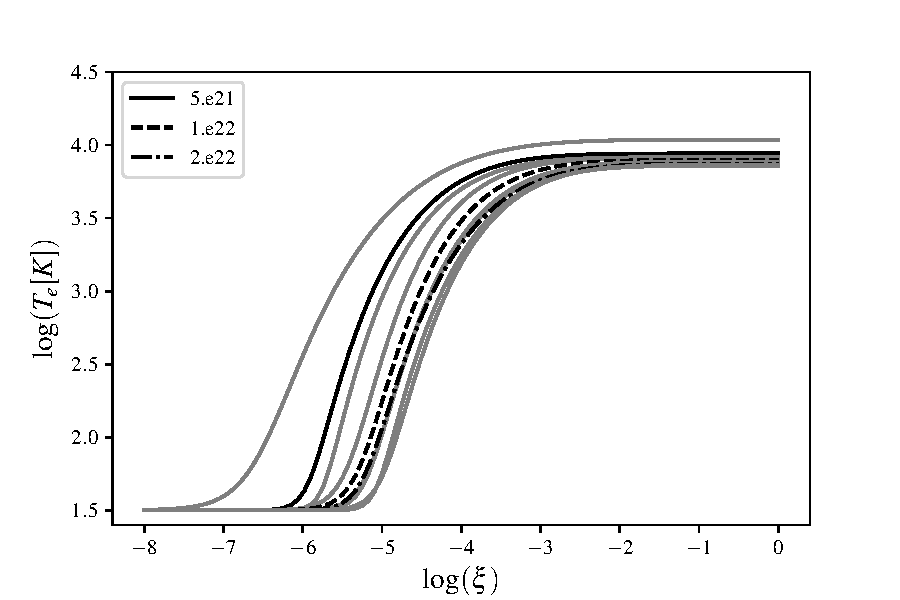
\includegraphics[width=.45\textwidth]{Fig1}
    \caption{Temperature as a function of the ionization parameter, where $3$ selected column densities are highlighted. \label{fig:tempxi}}
\end{figure}

The dust temperatures and initial density structure are calculated using the D’Alessio
Irradiated Accretion Disk (\textsc{DIAD}) radiative transfer models \citepads{1998ApJ...500..411D,1999ApJ...527..893D,2001ApJ...553..321D,2005ApJ...621..461D,2006ApJ...638..314D}, that best fit the median spectral energy distribution (SED) in Taurus.
The gas temperatures is assumed to be completely coupled to the dust temperature for $N>N_X$.

\begin{table*}
\caption{Star and disc properties}
\label{tab:stars}
\centering
\begin{tabular}{c c c c c c c c c}
\hline
$M_\star$ [$M_\odot$] & $R_\star$ [$R_\odot$] & ST & $L_\star$ [$L_\odot$] & $L_X$ [$10^{29}$ erg/s] & $T_\star$ [K] & M$_\mathrm{d}$ [$M_\odot$] ($\%$) & R$_{in}$ [au] & R [cells]\\
\hline
\hline
   $1.0$ & $2.615$ & K6 & $2.335$ & $20.4$ & $4278$ & $0.0444$ ($4.4$) & $0.445$ & $412$\\
   $0.5$ & $2.125$ & M1 & $0.9288$ & $7.02$ & $3771$ & $0.0363$ ($7.3$) & $0.2225$ & $449$\\
   $0.3$ & $2.310$ & M5 & $0.6887$ & $3.20$ & $3360$ & $0.0292$ ($9.7$) & $0.1335$ & $477$\\
   $0.1$ & $1.055$ & M6 & $0.08559$ & $0.589$ & $2928$ & $0.0264$ ($26.4$) & $0.0445$ & $535$\\
\hline
\end{tabular}
\end{table*}

\subsection{Hydrodynamical model}

We performed a set of hydrodynamical simulations using the \textsc{PLUTO} code \citepads{2007ApJS..170..228M}, adopting a spherical coordinate system centred on to the star.
The grid is logarithmically spaced in the radial direction, in order to have better resolution in the inner region of the disc, where photo-evaporation is mostly effective.
At the same time, it allows us to model the disc out to large radii ($R_{out}= 1000$ au) without increasing strongly our computational costs and preventing boundary effects that can affect the stability of the wind flow.
For a detailed discussion of the numerical artifacts induced by the grid outer boundary, the reader is referred to \citetads{2019MNRAS.487..691P}.
The grid is spaced linearly in the polar direction to maximize the resolution at the wind launching region.

We initially evolve the system for $100$ orbits at \si{10}{au} without stellar irradiation, in order to reach a quasi-hydrostatic equilibrium.
Then, we switch on the stellar heating (applied through a parameterisation from the radiative transfer simulation, as explained above) and continue to evolve the system until the cumulative mass-loss rate and gas streamline in the wind have reached a stable configuration.

%-------------------------------------------------------------------
\section{Results}
%-------------------------------------------------------------------

\subsection{Primordial discs}

We integrated the gas flow along the streamlines during the last 200 orbits of our simulations and plotted the result in a sqaure-box plot in Fig.~\ref{fig:Mdot}. A fitting function has been overplotted in black, which shows the steep dependance of the mass-loss rate for the lower end of stellar mass studied, while it becomes much flatter around few times $10^{-8}$ for $M_\star > 0.3 M_\odot$. This behavior is in contrast with the much shallower function derived in \citep{Owen2012}. We show in the plot that the fitting function obtained in O12 is still able to reproduce the only two value modelled in their study (i.e. 0.1 and 0.7 Solar mass stars).
The best fitting function obtained from the current study is
\begin{equation}
  \dot{M} = 2.56\times10^{-8} - 2.41\times10^{-9}\times\left(\frac{M_\star}{M_\odot}\right)^{-0.98},
\end{equation}
where one can see that the mass loss-rate is almost inversely proportional to the stellar mass.
In this analysis the dependance on the stellar X-ray luminosity is not considered, but the value adopted for the simulation is mass-dependant following the relation
\begin{equation}
	\log_{10}{(L_X)} = 1.54\times \log_{10}{(M_\star)} + 30.31
\end{equation}

\subsubsection{Mass-loss rates}
\begin{figure}
  \centering
  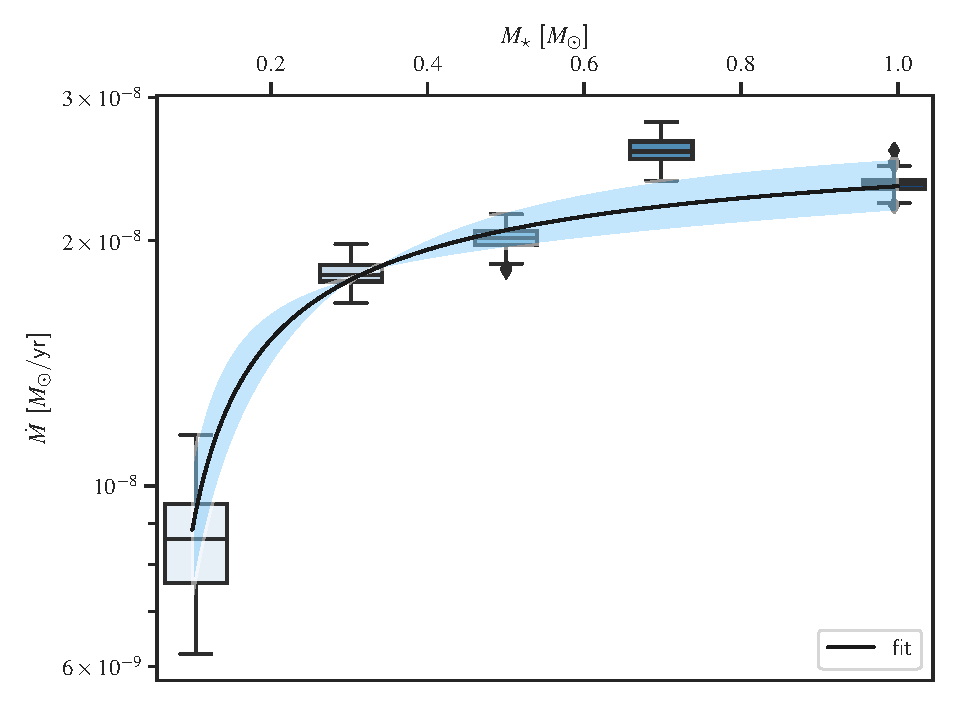
\includegraphics[width=0.45\textwidth]{mdot}
  \caption{Cumulative mass-loss rate as a function of stellar mass. \label{fig:Mdot}}
\end{figure}

\subsubsection{Wind profiles}
\begin{figure}
  \centering
  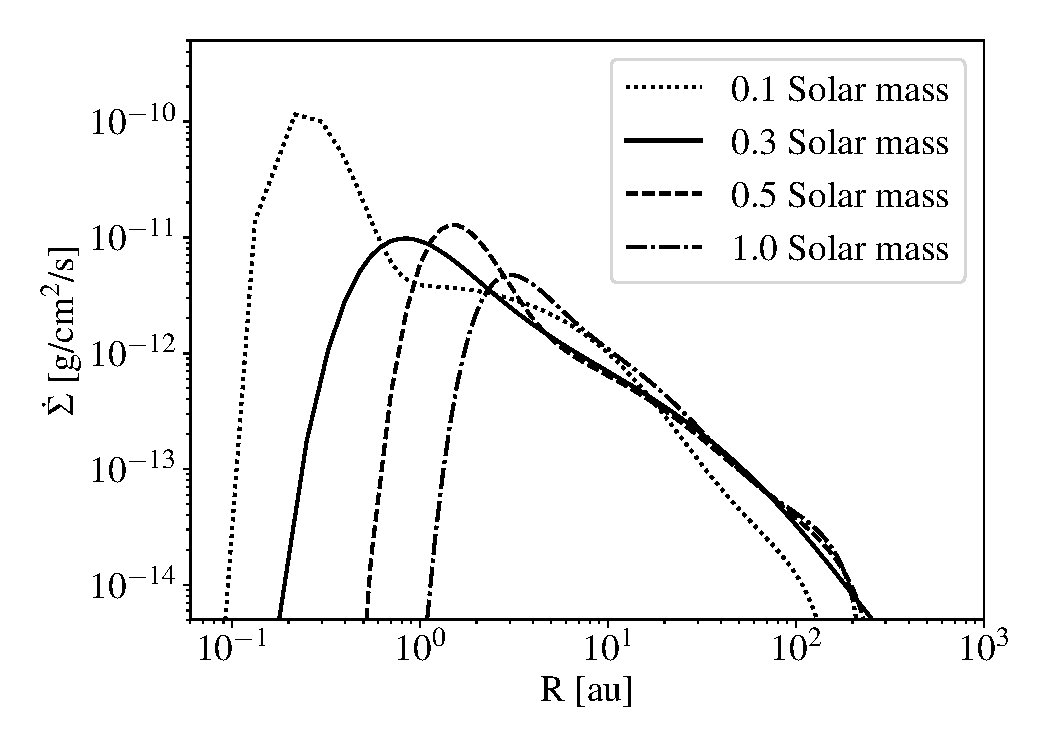
\includegraphics[width=0.45\textwidth]{Surfprofile}
  \caption{Surface density mass-loss rate profile for the different simulations. \label{fig:Sigmadot}}
\end{figure}

\subsubsection{Sonic surface}

The analysis of \citet{Owen2012} is based on the assumption that the properties of the mass-flux can be determined at the sonic surface, and that the sound speed is roughly given by the Parker value
\begin{equation}
  c_s^2 = \frac{GM_\star}{2R}
\end{equation}
An important assumption is that the height of the sonic surface is not much larger than its cylindrical radius ($z_s \ngg R$), which can brake down for lower stellar masses, since the disc flaring is proportional to the central mass.

%-------------------------------------------------------------------
\section{Conclusions}
%-------------------------------------------------------------------

   \begin{enumerate}
      \item PE exists.
   \end{enumerate}

\begin{acknowledgements}
    GP acknowledges support from the DFG Research Unit ‘Transition Disks’ (FOR 2634/1, ER 685/8-1).
    This work was performed on the computing facilities of the Computational Center for Particle and Astrophysics (C2PAP).
\end{acknowledgements}

\bibliographystyle{aa}
\bibliography{biblio}{}

\end{document}
